\documentclass[conference]{IEEEtran}
\IEEEoverridecommandlockouts

\usepackage{graphicx}
\usepackage{amsmath,amssymb}
\usepackage{cite}
\usepackage{tabularx}
\usepackage{amsmath,amssymb,amsfonts}
\usepackage{algorithmic}
\usepackage{graphicx}
\usepackage{textcomp}
\usepackage{xcolor}
\sloppy

\begin{document}

\title{Enhancing Educational Feedback: Development and Evaluation of a Real-Time Student Feedback System for Bangladeshi Universities\\


}

\author{\IEEEauthorblockN{ Mahmood Tauhidul}
\IEEEauthorblockA{\textit{Department of CSE} \\
\textit{Independent University Bangladesh}\\
Dhaka, Bangladesh\\
2010387@iub.edu.bd}
\and
\IEEEauthorblockN{ Rakib Ahmad}
\IEEEauthorblockA{\textit{Department of CSE} \\
\textit{Independent University Bangladesh}\\
Dhaka, Bangladesh\\
2130227@iub.edu.bd}
\and
\IEEEauthorblockN{ Simanto Saha}
\IEEEauthorblockA{\textit{Department of CSE} \\
\textit{Independent University Bangladesh}\\
Dhaka, Bangladesh \\
2130220@iub.edu.bd}
\and
\IEEEauthorblockN{Ahnaf Abdullah}
\IEEEauthorblockA{\textit{Department of CSE} \\
\textit{Independent University Bangladesh}\\
Dhaka, Bangladesh \\
2130223@iub.edu.bd}
}

\maketitle

\begin{abstract}
    The limitations of traditional course feedback mechanisms in Bangladeshi universities, particularly their end-of-semester timing and perceived ineffectiveness, underscore the need for innovative solutions. This research introduces a modernized course feedback system prototype, addressing these challenges through a systematic approach. The study begins with a comprehensive literature review to identify key issues, followed by a quantitative analysis of survey data collected from students and faculty to understand existing feedback practices and user needs. Employing a User-Centered Design (UCD) framework and iterative development methods, the system was designed using advanced web technologies, including Next.js and Shadcn UI. Key features of the prototype include real-time feedback progress tracking, course management capabilities, achievement systems, and impact visualization tools, all aimed at enhancing usability and engagement. Usability testing, conducted with 16 university students using the System Usability Scale (SUS), resulted in a score of 77.5\%, indicating strong user acceptance and system effectiveness. By combining advanced technology with a focus on user needs, this feedback system prototype demonstrates significant potential for improving educational feedback processes, setting a foundation for broader deployment and long-term assessment.
    \end{abstract}
    

    \begin{IEEEkeywords}
        Course Feedback, Usability Testing, Educational Technology, Privacy, Higher Education, Bangladesh
        \end{IEEEkeywords}

\section{Introduction}

In addition to various educational reforms, enhancing effective communication between students and faculty members plays a pivotal role in improving educational experiences and outcomes. Primarily, such communication occurs through the student feedback system, which enables students to share their perspectives on their learning journey while assisting instructors in reshaping their teaching strategies. Traditional feedback mechanisms, often restricted to end-of-semester evaluations, fail to provide sufficient timeliness or depth to facilitate real-time adjustments to course delivery. Consequently, there is a growing appreciation for more dynamic, interactive, and continuous feedback systems that offer immediate insights and foster ongoing conversations between students and educators.

With the rapid advancements in educational technology, many limitations of traditional feedback systems have been addressed through the introduction of new platforms. For instance, platforms such as OpineBot utilize conversational large language models to provide students with personalized feedback sessions, offering deeper and more actionable insights for instructors \cite{tanwar2024opinebotclassfeedbackreimagined}. Similarly, leveraging predictive models in feedback systems shows promise in improving the significance and quality of student assessments \cite{friedman2024enhancingstudentfeedbackusing}.

The objective of this investigation is to gain insights into the perceptions of individual faculty and students regarding existing feedback processes, as well as the challenges and preferences associated with them. The aim is to develop an improved course feedback system. Through comprehensive surveys targeting both groups, this research seeks to uncover current practices, perceived effectiveness, and desired features of feedback systems. As such, this study serves as an initial step toward creating a more responsive and user-centered feedback platform, aspiring to implement continuous improvements in higher education teaching and learning.


With advancements in generative AI, automated feedback systems are increasingly being adopted to address traditional feedback limitations, such as timeliness and personalization. Lindsay et al. \cite{lindsay2024responsibledevelopmentautomatedstudent} emphasize the importance of ethical frameworks in developing such systems, while Shi and Aryadoust \cite{Shi_Aryadoust_2024} provide a comprehensive overview of AI's role in written feedback tools.

The remainder of this paper describes the process used to collect data, analyzes the survey results, and provides recommendations for designing an improved course feedback system that meets the needs and expectations of both students and faculty.



\section{Related Works}

The development of effective feedback systems in higher education has garnered significant attention, with numerous studies highlighting the limitations of traditional methods and exploring innovative technological solutions to enhance student learning outcomes.

\subsection{Adaptive Assessments and Gamification in Feedback Systems}

Personalized learning platforms leverage AI to provide real-time adaptive assessments that cater to the unique needs of individual learners. These systems utilize predictive analytics and machine learning models to analyze student performance data, dynamically adjusting the complexity and content of assessments. This ensures a tailored learning experience, addressing areas where students need improvement while enhancing engagement. MDPI Electronics highlights the effectiveness of such platforms in creating adaptive feedback mechanisms that foster personalized learning experiences \cite{mdpi2024personalized}.

In addition to adaptive assessments, gamification strategies have gained significant attention as a means to improve student motivation and engagement. By incorporating elements such as badges, rewards, leaderboards, and progress tracking, gamification transforms the feedback process into an interactive and rewarding experience. These strategies encourage consistent participation in feedback activities, thereby providing instructors with more comprehensive and actionable data. Larrosa et al. \cite{electronics13183762} emphasize that gamified feedback systems serve as effective formative assessment tools, helping students stay motivated while fostering a sense of accomplishment.

The integration of adaptive assessments and gamification not only enhances the feedback experience for students but also provides educators with valuable insights into student progress. Such systems can significantly improve the quality of teaching and learning outcomes by bridging the gap between student needs and instructor interventions.

\subsection{Limitations of Traditional Feedback Mechanisms}

Traditional feedback methods, such as end-of-semester evaluations, often suffer from delays and lack the immediacy required for timely pedagogical adjustments. These methods may not provide the depth necessary to facilitate meaningful improvements in teaching and learning processes. For instance, a study evaluating challenges in delivering effective student feedback emphasizes the need for more immediate and actionable feedback to enhance student engagement and learning outcomes \cite{article1}.

\subsection{Advancements in Feedback Systems through Technology}

To address these challenges, researchers have explored technology-driven solutions that offer more dynamic and interactive feedback mechanisms.

\subsubsection{Predictive Analytics}

The integration of predictive analytics into educational feedback systems has shown promise in enhancing the quality and relevance of student assessments. By analyzing historical data, predictive models can forecast student performance, enabling educators to identify at-risk students and tailor interventions accordingly. A comprehensive review of predictive learning analytics over the past decade underscores its potential in improving educational outcomes \cite{Sghir2023}.

\subsubsection{Machine Learning Applications}

Machine learning techniques have been employed to predict student performance, providing insights that can inform personalized feedback and support. For example, a study utilizing machine learning-based predictive analytics demonstrated the effectiveness of such models in forecasting academic success, thereby facilitating timely interventions \cite{8725237}.

\subsubsection{Natural Language Processing (NLP)}

The application of NLP in analyzing student feedback has enabled the extraction of meaningful insights from qualitative data. This approach allows for a more nuanced understanding of student sentiments and experiences, informing targeted improvements in teaching strategies. A survey on student feedback assessment tools highlights the potential of NLP in handling and interpreting student feedback effectively \cite{edalati2020potentialmachinelearningnlp}.

\subsection{Conversational AI in Feedback Systems}

The advent of conversational AI tools has further revolutionized feedback processes by facilitating personalized and interactive feedback sessions.

\subsubsection{OpineBot}

Platforms like OpineBot leverage conversational agents to engage students in personalized feedback dialogues, providing instructors with actionable insights while enhancing student engagement. This approach underscores the value of AI in creating more responsive and user-centered feedback systems \cite{tanwar2024opinebotclassfeedbackreimagined}.

\subsection{Challenges and Future Directions}

Despite these advancements, challenges remain in ensuring the usability and effectiveness of feedback systems.

\subsubsection{Feedback Literacy}

Developing students' feedback literacy is crucial for maximizing the benefits of feedback systems. A recent study emphasizes the importance of equipping students with the skills to interpret and utilize feedback effectively, thereby enhancing learning outcomes \cite{Nieminen2023}.

\subsubsection{Integration of Predictive Models}

While predictive models offer valuable insights, their integration into existing educational frameworks requires careful consideration to ensure accuracy and relevance. A study on aligning learners' expectations and performance through predictive models highlights the need for user-centered design in developing effective learning analytics systems \cite{bdcc8120187}.

\subsection{Research Gap}

Current feedback systems in higher education, particularly those used for course evaluations, face several limitations that hinder their effectiveness in enhancing both teaching quality and student learning outcomes. These shortcomings include delayed feedback processing, limited engagement, and a lack of actionable insights from feedback data.

\subsubsection{Delayed Feedback Processing}

One of the primary limitations of traditional feedback systems is the delay in processing and delivering feedback. Most feedback systems, particularly those that rely on end-of-semester evaluations, provide feedback too late for instructors to make timely adjustments to their teaching strategies. This delay limits the ability to use feedback effectively in real-time to improve the learning experience.

\subsubsection{Limited Engagement and Interaction}

Another issue with current feedback systems is the lack of engagement between students and instructors. Traditional feedback methods often result in low response rates and may fail to capture meaningful insights. In many cases, feedback is treated as a one-way communication from students to faculty without fostering an ongoing dialogue. This limits the potential for feedback to drive real improvements in teaching methods and course content.

\subsubsection{Inefficient Data Analysis}

Current systems also face challenges in analyzing qualitative feedback data effectively. Manual analysis of free-text feedback is time-consuming and may miss underlying patterns or nuanced student sentiments. Without sophisticated tools to process and interpret this data, feedback may fail to provide instructors with the clear, actionable insights they need to make improvements.

\subsubsection{Scalability Concerns}

As class sizes increase, the ability to provide personalized, meaningful feedback diminishes. Many current systems are not scalable and struggle to provide personalized feedback at the individual student level, especially in large courses. This leads to a generalization of feedback that may not address the unique concerns or experiences of each student.

\subsubsection{Proposed Enhancements in the Prototype}

The feedback system presented in this prototype addresses these gaps by offering real-time feedback processing, interactive and personalized student-instructor communication, and efficient analysis of feedback data. By enabling students to provide feedback throughout the semester and allowing instructors to review and respond in real-time, the proposed system offers a dynamic and continuous feedback loop. Additionally, the system integrates tools for analyzing both quantitative and qualitative feedback, ensuring that instructors receive actionable insights that can drive meaningful improvements in their teaching practices. This research aims to bridge these gaps by creating a more responsive, engaging, and scalable feedback system for higher education.



\section{Design Requirement Elicitation}
\subsection{Study Design}

To evaluate the effectiveness of the enhanced course feedback system, surveys were conducted with both students and faculty members. The purpose of the surveys was to gather insights on current feedback practices, preferences for a new feedback system, and any challenges or concerns with existing mechanisms. The survey was designed to be comprehensive yet concise, allowing participants to provide both quantitative and qualitative responses.

\subsubsection{Survey for Students}
The student survey aimed to gather information about their demographics, feedback practices, preferences for the new system, concerns about privacy, and suggestions for improvements. The survey consisted of five sections:

\begin{itemize}
    \item \textbf{Section 1: Demographics} – This section collected basic demographic information such as the student's academic year and the number of courses they are currently enrolled in.
    \item \textbf{Section 2: Current Feedback Practices} – This section assessed how often students provide feedback, whether they feel their feedback is acted upon, and the challenges they face when providing feedback.
    \item \textbf{Section 3: Preferences for the New System} – This section inquired about the preferred frequency of feedback collection, the types of feedback formats, and the importance of various features such as anonymity, real-time responses, and mobile compatibility.
    \item \textbf{Section 4: Privacy and Security} – This section focused on students' concerns regarding the anonymity and confidentiality of their feedback.
    \item \textbf{Section 5: Open Suggestions} – This open-ended section allowed students to suggest features or improvements they would like to see in the feedback system.
\end{itemize}

\subsubsection{Survey for Faculty Members}
The faculty survey aimed to gather feedback on current practices, challenges, and preferences for a new feedback system. The survey consisted of the following sections:

\begin{itemize}
    \item \textbf{Section 1: Demographics} – This section asked faculty members how many courses they are teaching and their teaching experience.
    \item \textbf{Section 2: Current Feedback Practices} – This section asked about the frequency of reviewing student feedback, the effectiveness of the current process, and challenges faced in using feedback for course improvements.
    \item \textbf{Section 3: Preferences for the New System} – This section inquired about the preferred frequency of feedback collection, the type of feedback that would be most useful, and the importance of features such as dashboards for summarizing feedback and the ability to respond to student feedback.
    \item \textbf{Section 4: Privacy and Security} – This section explored concerns regarding how student feedback is presented to faculty members, and whether they prefer to respond to feedback anonymously or with their identity visible.
    \item \textbf{Section 5: Open Suggestions} – This open-ended section allowed faculty to provide suggestions for improving the feedback system.
\end{itemize}

\subsubsection{Data Collection and Analysis}
The surveys were distributed using an online platform, ensuring easy access for both students and faculty. The responses were analyzed quantitatively for multiple-choice questions and qualitatively for open-ended responses. This allowed us to identify trends in feedback preferences and areas for improvement in the feedback system.


\subsection{Data Collection Procedures}
Data for this study were gathered through surveys distributed using Google Forms. The online platform was selected to ensure easy access for both students and faculty, allowing them to complete the surveys at their convenience. Google Forms enabled the collection of both quantitative data (via multiple-choice questions) and qualitative data (via open-ended responses). The surveys were shared through direct links, and reminders were sent to encourage participation.



\subsection{Participants}
The study participants consisted of university students and faculty members. The demographics of the participants include a diverse group of individuals who are currently enrolled in various programs at the university, as well as faculty members with different levels of teaching experience.

\subsubsection{Demographics}
All participants were affiliated with the university. The student participants represented various academic years and fields of study, ensuring a broad range of perspectives on the current course feedback system. The faculty participants included instructors from different departments, with varying years of teaching experience.

\subsubsection{Selection Criteria}
The selection criteria for the study were straightforward: participants had to be university students or faculty members. Students were selected regardless of their academic year, while faculty participants were selected based on their involvement in teaching university-level courses. The study aimed to capture feedback from both groups to understand the feedback system’s effectiveness from multiple viewpoints—students' experiences and faculty members' use of the feedback for course improvement.


\subsection{Measures and Data Analysis}
The data collected from the surveys were analyzed using a combination of Excel and Google Forms' inbuilt data analysis tools. Google Forms automatically compiled the responses into a structured format, making it easy to view and organize the data. 

For quantitative data, such as multiple-choice responses, basic statistical techniques were applied, including frequency counts and percentage distributions, to identify patterns and trends in student and faculty feedback. Excel was used to perform more detailed analysis, including the generation of graphs and charts to visually represent the data, as well as calculations for means and standard deviations where applicable.

For qualitative data, such as open-ended responses, thematic analysis was conducted to identify common themes and sentiments expressed by participants. The responses were manually reviewed to group similar comments and categorize them into relevant themes, providing deeper insights into the preferences, challenges, and suggestions of both students and faculty members.

By combining both quantitative and qualitative analysis, the study aimed to provide a comprehensive understanding of the current feedback system and areas for improvement.


\subsection{Findings Based on RQs}

\subsubsection{RQ1: What are the current feedback practices of students and faculty members?}
Based on the survey responses, it was found that the majority of students (77.4\%) submit feedback only at the end of the semester, while a smaller proportion (12.9\%) provide feedback periodically throughout the semester. Only 9.7\% of students indicated that they never provide feedback.

\begin{figure}[htbp]
    \centering
    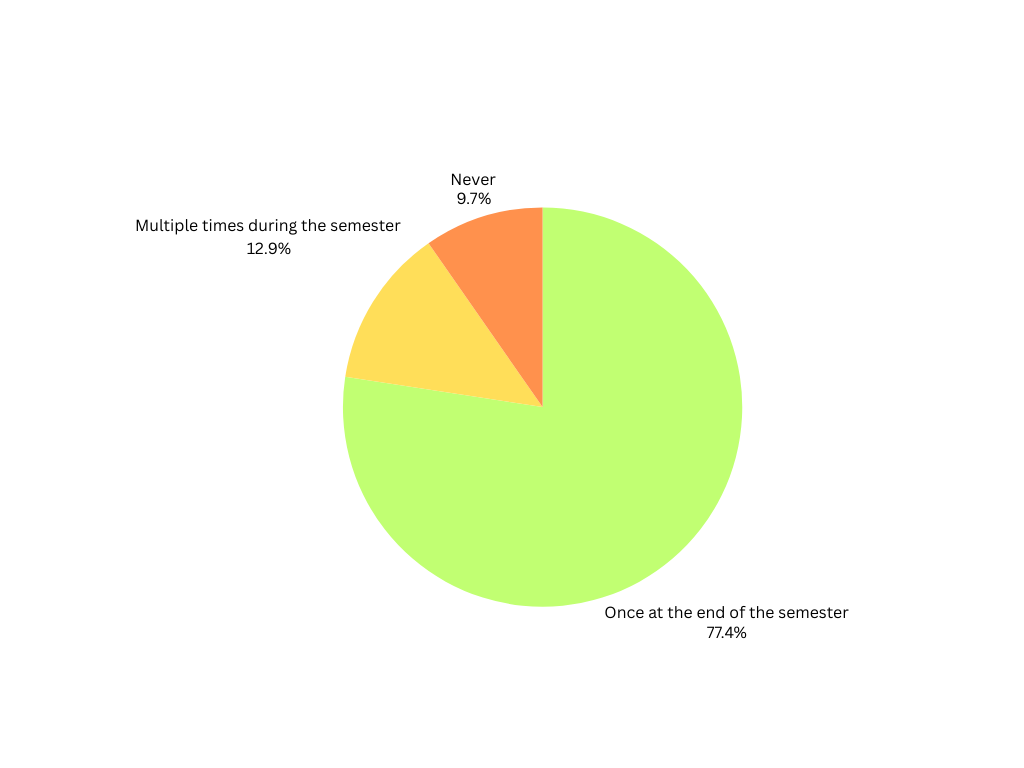
\includegraphics[width=0.8\linewidth]{feedback_practices.png}
    \caption{Feedback practices of students}
    \label{fig:feedback_practices}
\end{figure}



\subsubsection{RQ2: How do students perceive the effectiveness of the current feedback system?}
The majority of students (48.4\%) expressed that they feel their feedback is often ignored or not acted upon. However, 35.5\% of students felt they werent sure if their feedback was acted upon. Only 16.1\% of students were confident that their feedback led to tangible changes in the course structure or teaching methods. These results suggest that students are generally dissatisfied with the responsiveness of the current feedback system.

\begin{figure}[htbp]
    \centering
    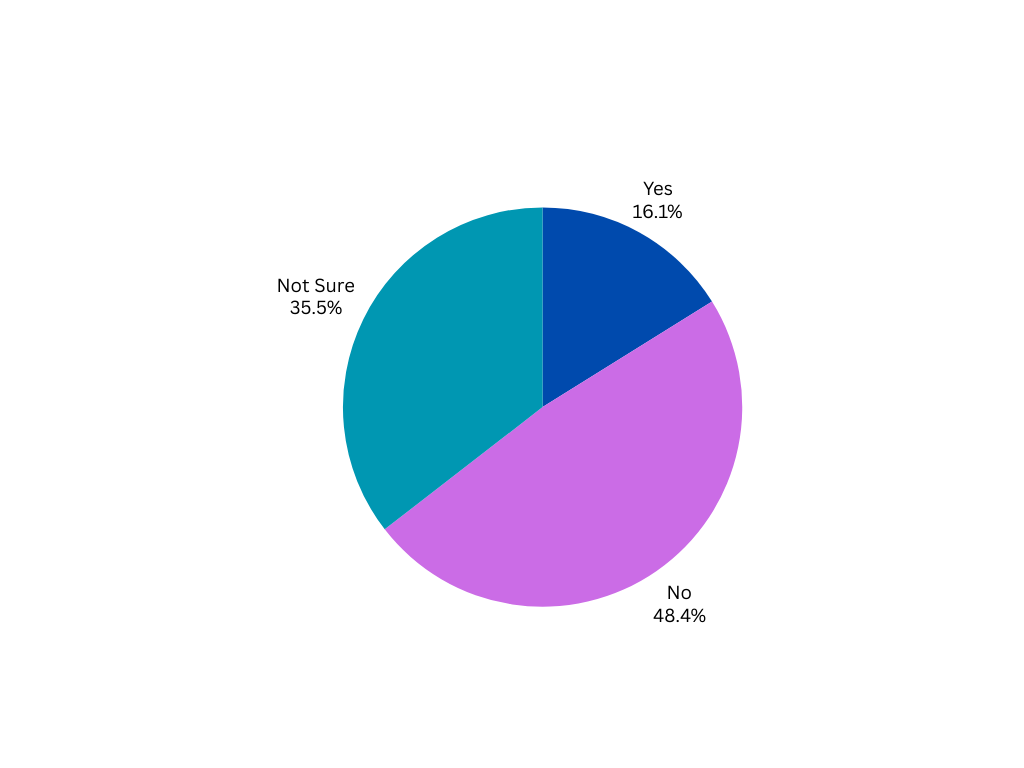
\includegraphics[width=0.8\linewidth]{feedback_action.png} 
    \caption{Student responses on the effectiveness of the current feedback system}
    \label{fig:feedback_action}
\end{figure}


\subsubsection{RQ3: What are the preferences of students for an improved feedback system?}
Students indicated a preference for more frequent feedback collection. Students favored receiving feedback monthly (45.2\%) or weekly (16.1\%).

\begin{figure}[htbp]
    \centering
    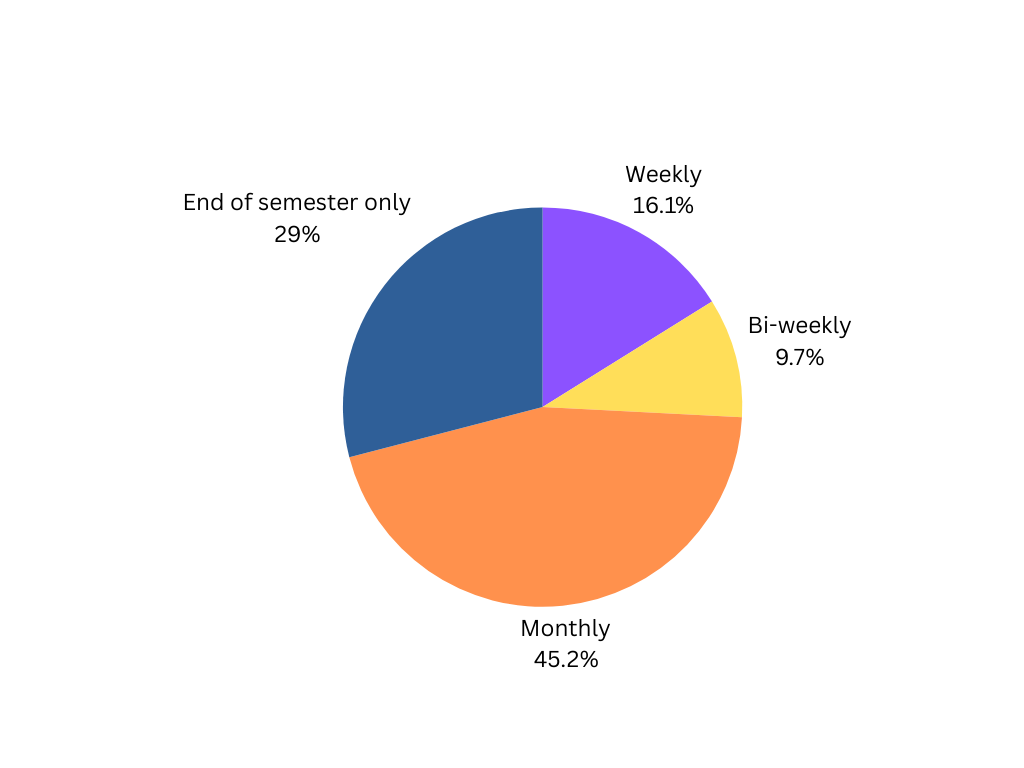
\includegraphics[width=0.8\linewidth]{feedback_report.png} 
    \caption{Student preferences for the frequency of feedback collection}
    \label{fig:feedback_report}
\end{figure}


\subsubsection{RQ4: How do privacy and security concerns influence students' willingness to provide feedback?}
When asked about concerns regarding anonymity, 10 students (32.3\%) expressed worries about their feedback being traced back to them, indicating significant concerns about privacy. However, 17 students (54.8\%) stated that they would feel more comfortable providing feedback if the system ensured full anonymity. In contrast, 5 students (16.1\%) felt that the level of anonymity in the current system was sufficient, expressing little to no concern. 

These findings suggest that a majority of students would be more willing to participate in the feedback process if privacy measures were enhanced. This highlights the importance of ensuring anonymity to increase engagement in feedback systems.
\begin{figure}[htbp]
    \centering
    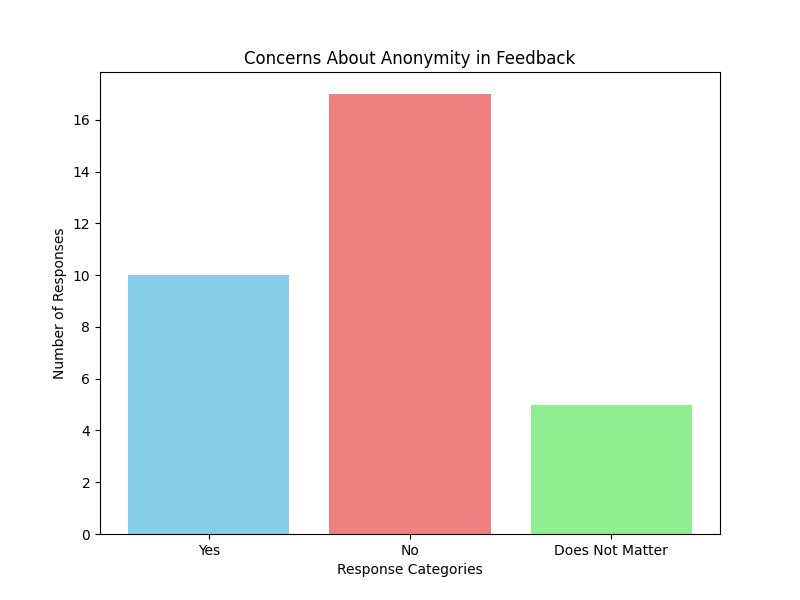
\includegraphics[width=0.8\linewidth]{feedback_anon.png} 
    \caption{Distribution of student concerns regarding anonymity in the feedback process}
    \label{fig:feedback_anon}
\end{figure}

\section{Prototype Design and Development}

The development of the course feedback system involved careful selection and integration of modern web technologies and frameworks.

\subsection{Development Environment and Tools}

Visual Studio Code (VS-Code) served as the primary integrated development environment, providing comprehensive development support through its extensive plugin ecosystem and efficient code editing capabilities.

\subsection{Frontend Framework and UI Components}

The frontend architecture leverages:
\begin{itemize}
    \item \textbf{Next.js Framework:} 
    \begin{itemize}
        \item \textbf{Server-side Rendering:} Optimized for performance and SEO.
        \item \textbf{Built-in Routing:} Simplified navigation and URL handling.
        
    \end{itemize}
    
    \item \textbf{UI Libraries:}
        \begin{itemize}
            \item \textbf{Shadcn UI:} For consistent form handling, modern interface components, and responsive design.
            \item \textbf{Aceternity UI:} For enhanced animations and interactive user interface elements.
        \end{itemize}
\end{itemize}

\subsection{Data Visualization Components}

The system incorporates:
\begin{itemize}
    \item \textbf{Chart.js:} For creating interactive and responsive charts for data analysis.
    \item \textbf{Matplotlib:} For generating complex statistical visualizations and data analysis representations.
\end{itemize}

\subsection{Development Methodology}

The development process followed an iterative approach, including:
\begin{itemize}
    \item Initial planning and requirement analysis
    \item Component-based development using Next.js
    \item Integration of UI libraries and form handling components
    \item Implementation of data visualization features
    \item Continuous testing and refinement
\end{itemize}

\begin{figure*}[htbp]
    \centering
    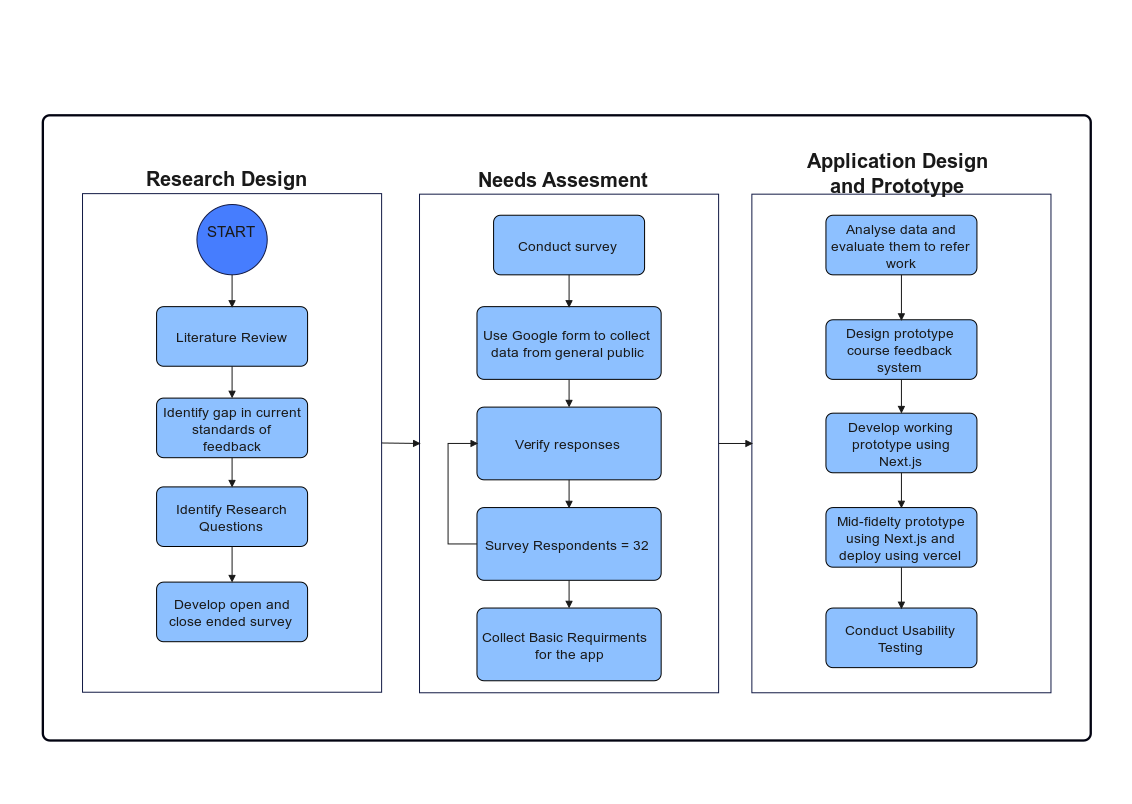
\includegraphics[width=0.8\linewidth]{research_workflow.png} 
    \caption{Research methodology describes 3 steps that were followed to develop the semester course feedback system, research design, need-finding,
    application design and development}
    \label{fig:research_workflow}
\end{figure*}

\begin{figure}[htbp]
    \centering
    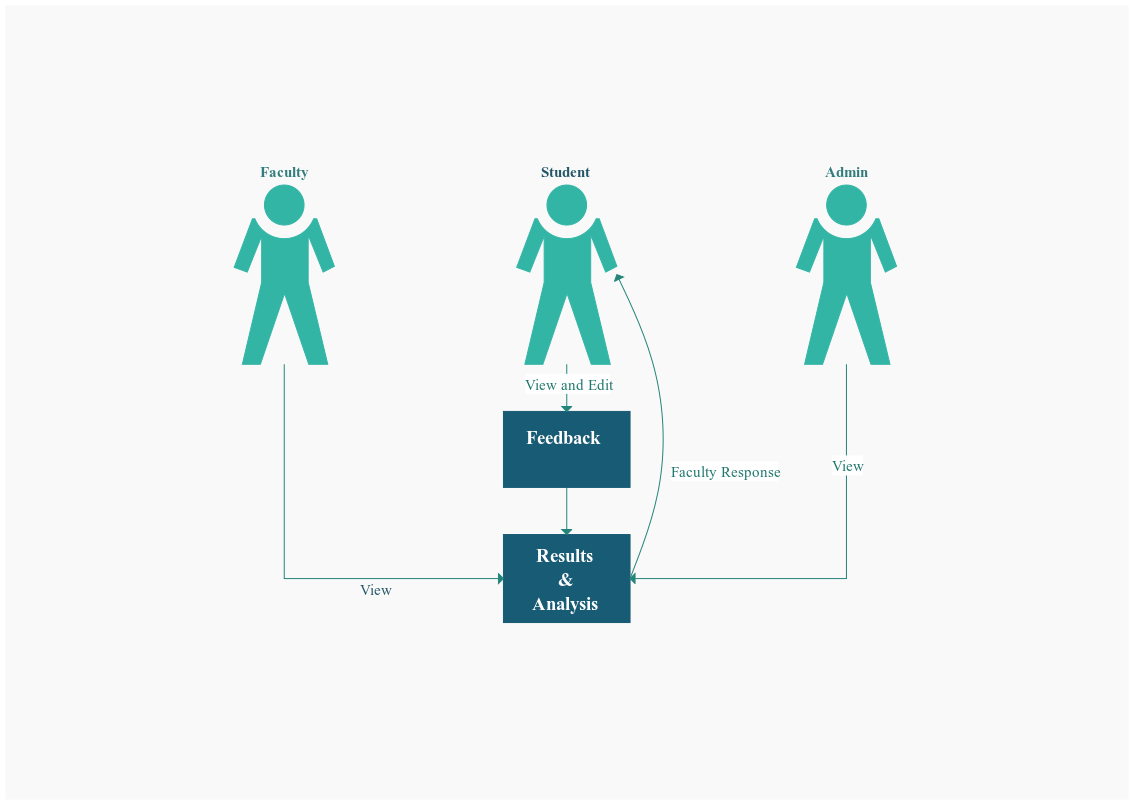
\includegraphics[width=0.8\linewidth]{data_flow.png} 
    \caption{Data flow diagram for the prototype}
    \label{fig:data_workflow}
\end{figure}

\section{Available Features}

The course feedback system offers a comprehensive set of features for both student and faculty portals.

\subsection{Student Portal Features}
\begin{itemize}
    \item \textbf{Feedback Progress Tracking: } Progress indicators for each course, feedback submission status, and last feedback date tracking.
    \item \textbf{Course Management:} List of enrolled courses, submission status, and last feedback date tracking.
    \item \textbf{Achievement System:} Badges for completing feedback, providing detailed feedback on course performance and engagement.
    \item \textbf{Impact Tracking:} Timeline of implemented changes based on student feedback.
\end{itemize}

\subsection{Faculty Portal Features}
\begin{itemize}
    \item \textbf{Course-Specific Analytics:} Monthly feedback overview, response tracking, and detailed analytics dashboards.
    \item \textbf{Data Visualization:} Rating trends, course pace distribution, and activities effectiveness analysis.
    \item \textbf{Response Management:} Toggle between analytics and individual responses, historical data tracking, and submission count tracking.
\end{itemize}

\subsection{Cross-Portal Features}
\begin{itemize}
    \item \textbf{User Profiles:} Semester identification, personal progress tracking, and achievement monitoring.
    \item \textbf{Navigation:} Intuitive tab-based navigation, clear status indicators, and easy access to historical feedback data.
\end{itemize}

\section{User Experience and Usability Evaluation}
\subsection{Study Design}

\section{Usability Evaluation}

A user-centered approach was adopted to assess the usability and user experience of the developed course feedback system prototype. A usability testing method was employed to evaluate the system's effectiveness in engaging users and providing actionable insights.

Gamification techniques, such as achievement badges and progress tracking, have been shown to significantly improve student engagement and motivation. These elements were integrated into the prototype to foster a more interactive and rewarding feedback process. Research from Frontiers in Education highlights the effectiveness of gamified systems in promoting sustained participation and improving overall user experience \cite{10.3389/feduc.2024.1466926}.

Participants completed predefined tasks, including navigating course pages, submitting feedback, and accessing analytics. Their experiences were measured using the System Usability Scale (SUS), and qualitative feedback was gathered through open-ended questions to identify areas for improvement.

The results indicate that integrating gamification elements alongside intuitive design contributes positively to user engagement, supporting findings from related research \cite{10.3389/feduc.2024.1466926}.

\begin{figure*}[!h]
    \centering
    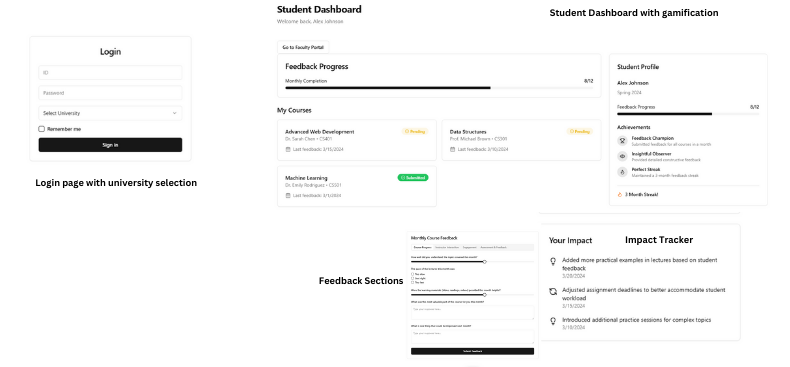
\includegraphics[width=\textwidth]{features.png}
    \caption{An illustrative collage representing the course feedback system features for students, including login.}
    \label{fig:student_features}
\end{figure*}

\begin{figure*}[!h]
    \centering
    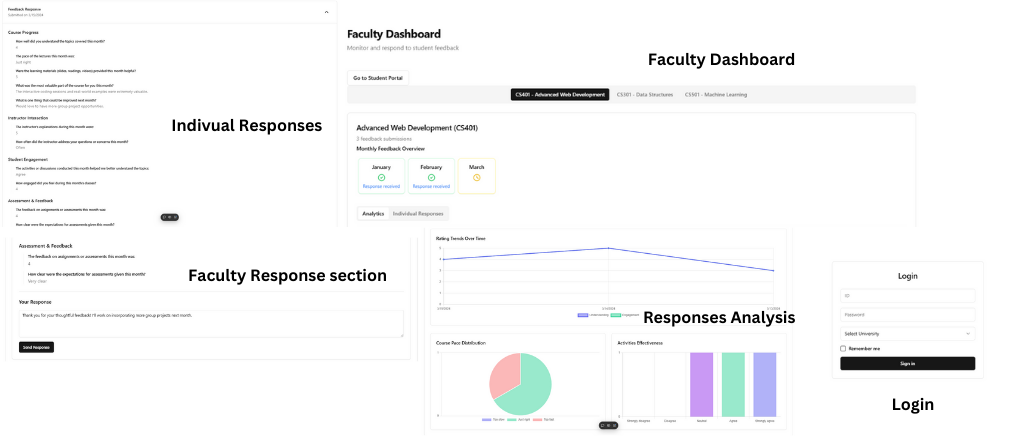
\includegraphics[width=\textwidth]{faculty.png}
    \caption{An illustrative collage representing the course feedback system features for faculties, including login.}
    \label{fig:faculty_features}
\end{figure*}



\subsection{Data Collection Procedures}
The online survey, conducted via Google Forms, was used to collect user feedback on the prototype system, particpants were invited to complete a series of tasks using the prototype system. They were asked to contribute voluntarily and were ensured about the confidentiality of their responses.
Task Definition: A set of predefined tasks was designed to assess the usability of the prototype system. These tasks included:
     Task 1: Navigating to a specific course page.
    Task 2: Submitting feedback for a course.
     Task 3: Viewing feedback history.
     Task 4: Accessing and understanding course-specific analytics. 
User Testing:Participants were individually guided through the testing process. They were instructed to complete the predefined tasks using the prototype system while "thinking aloud," verbalizing their thoughts and actions. This "think aloud" protocol helped to identify any usability issues or areas of confusion.


\subsection{Participants}
A convenience sample of 16 university students was recruited to participate in the usability evaluation. Participants were selected based on their availability and willingness to participate in the study. The participants included students from different academic programs and years of study, ability to read and speak in English and had minimum experience with feedback systems and smart devices including desktops,laptops and smartphones.

\subsection{Measures and Data Analysis}
Quantitative data, such as task completion times and user satisfaction ratings, were analyzed using descriptive statistics (e.g., means, standard deviations). User satisfaction was further assessed using the System Usability Scale (SUS), a 10-item questionnaire measuring user perceptions of system usability. The SUS score is calculated using the following formula:

\begin{equation*}
SUS = \frac{\sum_{i=1}^{10} (Q_i - 1) * 4}{10} * 100
\end{equation*}

where:

* $Q_i$ represents the user's response to each question on the SUS scale (1-5).
To evaluate the usability of the system, we employed the System Usability Scale (SUS). The SUS consists of ten statements to which participants respond on a 5-point Likert scale ranging from "Strongly Disagree" to "Strongly Agree." Each response is converted into a score from 0 to 4, where:

\begin{itemize}
    \item For odd-numbered statements, the score is the response minus 1.
    \item For even-numbered statements, the score is 5 minus the response.
\end{itemize}

The following table presents the responses, means, and the converted SUS scores:

Qualitative data from the open-ended questions were analyzed using thematic analysis to identify common themes and patterns in user feedback. 
\begin{table}[ht]
    \centering
    \caption{System Usability Scale (SUS) Results}
    \begin{tabular}{l|ccccc|c}
    \hline
    \textbf{Statement} & \textbf{SD} & \textbf{D} & \textbf{N} & \textbf{A} & \textbf{SA} & \textbf{Mean} \\ \hline
    I would use system frequently. & 1 & 0 & 1 & 3 & 10 & 4.125 \\
    System is complex. & 10 & 2 & 0 & 2 & 1 & 1.75 \\
    System is easy to use. & 1 & 0 & 0 & 3 & 11 & 4.375 \\
    May need technical help. & 9 & 5 & 0 & 0 & 1 & 1.50 \\
    Functions well integrated. & 1 & 0 & 2 & 6 & 6 & 3.875 \\
    System consistent in design. & 1 & 0 & 0 & 7 & 7 & 4.125 \\
    Learn to use quickly. & 1 & 0 & 1 & 5 & 8 & 4.125 \\
    System is cumbersome. & 13 & 0 & 0 & 1 & 1 & 1.125 \\
    Confident using system. & 1 & 0 & 0 & 9 & 5 & 4.00 \\
    Requires much learning. & 12 & 0 & 1 & 1 & 1 & 1.25 \\ \hline
    \multicolumn{6}{c|}{77.5\% SUS Score} & \\ \hline
    \end{tabular}
    \label{tab:sus_results}
    \end{table}

    The SUS score was calculated as follows:
    \begin{enumerate}
        \item Convert each mean response to a SUS score:
        \begin{itemize}
            \item Odd-numbered questions: Mean - 1
            \item Even-numbered questions: 5 - Mean
        \end{itemize}
        \item Sum the converted scores:
        \begin{align}
            &3.125 \approx 3,& \ 3.25 \approx 3,& \ 3.375 \approx 3,& \ 3.5 \approx 4, \nonumber \\
            &2.875 \approx 3,& \ 0.875 \approx 1,& \ 3.125 \approx 3,& \ 3.875 \approx 4, \nonumber \\
            &3.00 \approx 3,& \ 3.75 \approx 4. \nonumber
        \end{align}
        \begin{equation}
            Sum = 3 + 3 + 3 + 4 + 3 + 1 + 3 + 4 + 3 + 4 = 31
        \end{equation}
        \item Multiply the sum by 2.5 to get the SUS score:
        \begin{equation}
            SUS\ Score = 31 \times 2.5 = 77.5\%
        \end{equation}
    \end{enumerate}
    \subsection{Findings}

    The usability evaluation conducted using the System Usability Scale (SUS) revealed several key insights into the user experience of the system:
    
    \begin{itemize}
        \item \textbf{Overall Usability Score:} The system received a SUS score of \textbf{77.5\%}, categorized as "Good" on the SUS scale, indicating generally positive user perceptions of system usability.
        \item \textbf{Frequent Use Preference:} With a mean score of 4.125 for the statement ``I think that I would like to use this system frequently,'' there is a strong positive inclination towards using the system regularly, suggesting that users find it engaging or useful for their needs.
        \item \textbf{System Complexity}: The statement ``I found the system unnecessarily complex'' had a mean score of 1.75, indicating that while some users perceived minor complexities, the majority did not find the system overly difficult to use.
        \item \textbf{Ease of Use}: A high mean score of 4.375 for ``I thought the system was easy to use'' reflects a consensus among users that the system interface is intuitive and straightforward.
        \item \textbf{Technical Support Needs:} A low mean score of 1.50 for ``I might need help from a technical person to use this system'' shows that most users feel they can navigate the system without extensive technical support, indicating good self-sufficiency in usage.
        \item \textbf{Integration of Functions}: The statement ``I found the various functions in this system were well integrated'' scored 3.875, suggesting that users generally perceive the system's components as working well together.
        \item \textbf{Design Consistency}: With a mean of 4.125 for ``I found the system consistent in its design,'' users appreciate the uniformity and predictability of the system's interface.
        \item \textbf{Learning Curve}: The low score of 1.25 for ``I needed to learn a lot of things before I could get going with this system'' implies that the system has a relatively gentle learning curve, allowing users to become operational quickly.
        \item \textbf{Confidence in Use}: A mean score of 4.00 for ``I felt very confident using the system'' points to a high level of user confidence, which is crucial for ongoing engagement and satisfaction.
        \item \textbf{Cumbersomeness}: With a mean of 1.125 for ``I found the system very cumbersome to use,'' it's clear that the system does not impose a significant burden on users, enhancing the positive user experience.
    \end{itemize}
    
    

\section{Limitations}
    In conducting this study, several limitations were encountered that could impact the robustness and generalizability of the findings:
    
    \begin{itemize}
        \item \textbf{System Availability}: The primary limitation was the inability to use a fully operational system for the usability testing. Participants interacted with a prototype or a partially implemented version of the system, which might not fully reflect the experience of using a complete, running application. This could have influenced the SUS scores and user feedback, potentially skewing perceptions of usability and functionality.
    
        \item \textbf{Sample Size and Diversity}: Another constraint was the limited reach in participant recruitment. We were unable to engage a broader spectrum of students and faculty members, which might have introduced bias in the sample. The diversity in terms of age, technical background, and familiarity with similar systems was not as varied as it could have been, thus possibly not representing the full range of potential users' experiences and needs.
    \end{itemize}
    
    \subsection{Areas for Improvement in Future Research}
    To address these limitations and enhance the quality of future studies, the following areas could be targeted for improvement:
    
    \begin{itemize}
        \item \textbf{Use of a Fully Functional System}: Conducting the study with a fully operational system would provide more accurate and comprehensive user feedback. This would allow for a more realistic assessment of usability, performance, and user satisfaction in real-world scenarios.
    
        \item \textbf{Expanded Participant Recruitment}: Future research should aim to involve a larger and more diverse sample of participants. This could include reaching out to different departments, academic levels, and even external institutions to capture a broader user base. Employing varied recruitment methods like online surveys, university-wide announcements, or even international partnerships could help in this regard.
    
        \item \textbf{Longitudinal Studies}: Implementing longitudinal studies would allow for the collection of data over an extended period, providing insights into how user perceptions and system usability evolve with time. This could reveal aspects like learning curves, long-term satisfaction, and the system's adaptability to user needs.
    
        \item \textbf{Incorporating More Quantitative and Qualitative Data}: Enhancing the study with additional quantitative metrics (like task completion times, error rates) alongside qualitative feedback through interviews or focus groups could yield a more nuanced understanding of the system's usability. 
    
        \item \textbf{Technological Enhancements}: Future studies could benefit from using advanced data collection tools or automated analysis software to handle feedback more efficiently, especially in large-scale implementations where manual processing might be prohibitive.
    
        \item \textbf{Cross-Platform Evaluation}: If the system is intended for use across different platforms (e.g., mobile, desktop), future research should ensure usability is tested across all relevant platforms to confirm consistent user experience.
    
        \item \textbf{Feedback Loop Implementation}: Incorporating mechanisms for ongoing user feedback post-launch could help in iterative system improvements based on real user experiences, enhancing both the system and the research process.
    \end{itemize}

    \section{Conclusion and Future Work}

In this research, we have advanced the course feedback system within Bangladesh's universities by implementing a more improved and continuous feedback mechanism. Our contributions include developing a system that facilitates real-time feedback processing, interactive communication, and sophisticated data analysis, with the goal of enhancing teaching quality and student learning outcomes. The System Usability Scale (SUS) was utilized to assess the system's usability, resulting in a commendable score of 77.5\%, although it indicates there is still potential for enhancement. We've also gathered insights on user engagement, suggesting a preference for frequent use and a low demand for technical support, which points to the system's user-friendliness.

Ethical considerations are paramount when scaling feedback systems, particularly those leveraging generative AI technologies. Lindsay et al. \cite{lindsay2024responsibledevelopmentautomatedstudent} emphasize the need for responsible development frameworks to ensure fairness, transparency, and privacy. As the system evolves, these principles will be integrated to maintain trust and accountability in AI-driven feedback mechanisms.

Future work will focus on fully deploying the system in a variety of Bangladeshi universities to evaluate its real-world impact. Broadening the participant base to include more diverse groups from various academic disciplines and institutions will ensure the system meets varied educational needs. Longitudinal studies should be conducted to assess the long-term effects on teaching practices and student performance, capturing changes in user interaction over time.

Additionally, integrating advanced gamification features, such as dynamic leaderboards and personalized achievement systems, will further enhance user engagement. Research from Frontiers in Education \cite{10.3389/feduc.2024.1466926} underscores the effectiveness of gamification in fostering sustained participation and improving learning outcomes. Employing these strategies will create a more interactive and rewarding experience for users, encouraging continuous feedback submission.

Integrating the system with existing educational data systems could enhance data analytics and personalize feedback further. Employing more advanced data analysis methods can extract deeper insights from feedback, leading to more targeted improvements in course delivery. Continuous refinement of the user interface based on ongoing user feedback will maintain its intuitiveness and adaptability to different user groups and technological environments.

Finally, investigating the system's direct impact on educational outcomes will affirm its pedagogical effectiveness. By addressing these areas, the system can evolve into a scalable, ethical, and engaging platform that transforms the feedback process in higher education, contributing significantly to the development of educational technologies tailored for Bangladesh's unique educational landscape.


\bibliographystyle{IEEEtran}
\bibliography{references}

\end{document}
